\documentclass[aps,twocolumn]{revtex4-1}

\usepackage{amsfonts}
\usepackage{amsmath}
\usepackage{geometry}
\usepackage{xcolor}
\usepackage{graphicx}
%\usepackage[subfolder,cleanup]{gnuplottex}
%\usepackage{amsthm}
%\usepackage{enumitem}
%\usepackage{wrapfig}
%\usepackage{subcaption}
%\usepackage{hyperref}
\usepackage{tikz}
\usepackage{lipsum}

% Nicer brackets for operators
\let\originalleft\left
\let\originalright\right
\renewcommand{\left}{\mathopen{}\mathclose\bgroup\originalleft}
\renewcommand{\right}{\aftergroup\egroup\originalright}

% Math operators
\providecommand{\bigO}[1]{\ensuremath{\mathop{}\mathopen{}\mathcal{O}\mathopen{}\left(#1\right)}}

% Macros
\newcommand{\diff}[3][\hspace{-0.5pt}]{\frac{\textrm{d}^{#1}#2}{\textrm{d}{#3}^{#1}}}
\newcommand{\pdiff}[3][\hspace{-0.5pt}]{\frac{\partial^{#1}#2}{\partial{#3}^{#1}}}
\newcommand{\df}{\, \textrm{d}}
%\newcommand{\eps}{\varepsilon}

% Row colouring in tables
%\usepackage[table]{xcolor}
%\rowcolors{2}{gray!25}{white}

% Margin size
\newgeometry{margin=2cm}

% Reference style
%\bibliographystyle{ieeetr}

\begin{document}

\title{Predicting NCAA March Madness 2019 with SpringRank}
\author{Brady Metherall}
\affiliation{University of Oxford}
\date{16 March, 2020}

\maketitle

Each spring the National Collegiate Athletic Association (NCAA) hold a single-elimination tournament across the United States known as March Madness. The top 68 US college basketball teams in Division I take part, with the winner being crowned the national champion. The champions of each of the 32 Division I conferences automatically included, and the remaining 36 spots are determined by a selection commitee.

We use the box scores of *** 6000 NCAA games before March Madness 2019 \cite{wirth}; this data contains 649 teams from all three divisions. From this, we build our directed adjacency matrix, where each game is represented by an edge from the winner to the loser.



\lipsum[1-3]

\begin{figure}[tb]
	\centering
	\begin{tikzpicture}
		\centering
		\node[anchor=south west,inner sep=0] at (0,0) {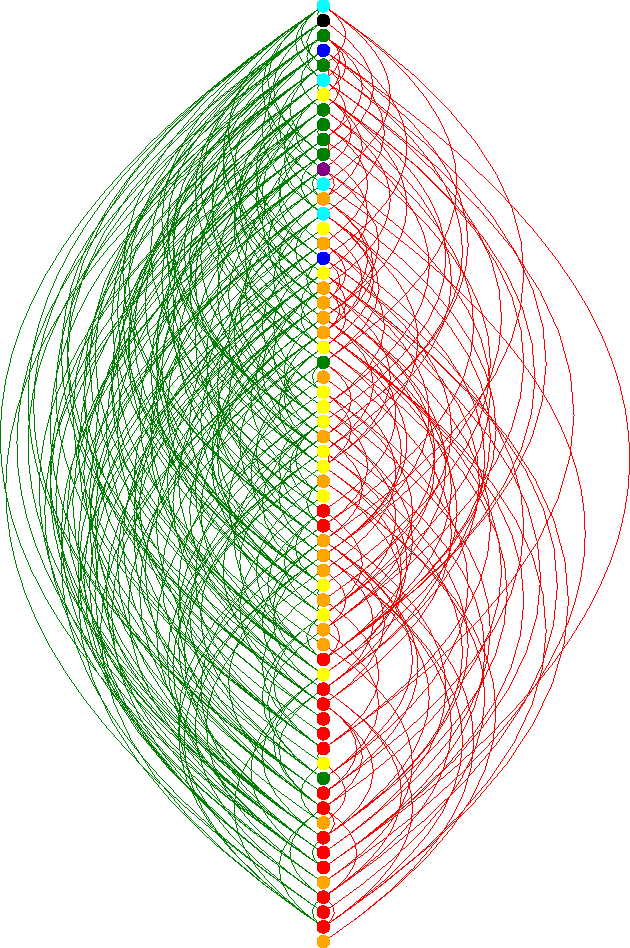
\includegraphics[width=0.66\columnwidth]{Heirarchy}};

		\fill[fill = black] (0.15,1) circle (0.6mm);
		\fill[fill = {rgb,255:red,128; green,0; blue,128}] (0.15,0.667) circle (0.6mm);
		\fill[fill = blue] (0.15,0.333) circle (0.6mm);
		\fill[fill = {rgb,255:red,0; green,255; blue,255}] (0.15,0) circle (0.6mm);

		\node[anchor = west] at (0.25,1) {\scriptsize Winner};
		\node[anchor = west] at (0.25,0.667) {\scriptsize Runner-up};
		\node[anchor = west] at (0.25,0.333) {\scriptsize Final four};
		\node[anchor = west] at (0.25,0) {\scriptsize Elite eight};

		\fill[fill = {rgb,255:red,0; green,128; blue,0}] (4.65,1) circle (0.6mm);
		\fill[fill = yellow] (4.65,0.667) circle (0.6mm);
		\fill[fill = {rgb,255:red,255; green,165; blue,0}] (4.65,0.333) circle (0.6mm);
		\fill[fill = red] (4.65,0) circle (0.6mm);

		\node[anchor = west] at (4.75,1) {\scriptsize Sweet 16};
		\node[anchor = west] at (4.75,0.667) {\scriptsize Round of 32};
		\node[anchor = west] at (4.75,0.333) {\scriptsize Round of 64};
		\node[anchor = west] at (4.75,0) {\scriptsize Did not qualify};
	\end{tikzpicture}
	\caption{Top 64 teams from SpringRank and their progress in March Madness 2019. A green (red) edge denotes the higher (lower) ranked team beat the lower (higher) ranked team during the season.}
	\label{fig:heir}
\end{figure}

\lipsum[1-2]
 \cite{debacco}
 \cite{wirth}
 \cite{vanderkam}

\bibliography{Ref}

\end{document}
